\chapter{Our Approach}
\label{chap:ourapp}


%In this chapter, we propose a novel approach to evaluate $k$GTP queries. In a $k$GTP query, the group provides the source and destination locations of the group members, $k$, and the required categories of POIs and the query returns $k$ sets of POIs as answer. Road networks are enormous in size with numerous POIs and the operation on all POIs brings huge processing overhead. The underlying idea of our approach is to refine the search space to reduce the number of POIs to be considered. The steps of our solution are as summarized as follows:


During building up the main approach, it is observed that spatial alarm evaluation can be optimized using three key features: 
\begin{itemize}
\setlength\itemsep{0em}
\item Firstly, reducing the number of device wake-ups;
\item Secondly, reducing any re-computation;
\item Thirdly, reducing the data communication overhead between the server and the client.
\end{itemize}

For the first strategy to be successful, we propose an algorithm in this section which will compute an optimal safe-region. The second optimization technique is realized by passing optimal parameters among different functions as well as between the client and the server, while the third one is achieved by passing minimal parameters between the client and the server and in some cases recomputing some values in each side.

However, the second and the third options have some conflicts in some cases and therefore cannot be achieved simultaneously. For this reason, we have separated some parts of our main approach within two different modes, namely - \textit{Bandwidth Saving (BWS) Mode} and \textit{Computational Cost Saving (CCS) Mode}.
\vspace{5pt}
In Section~\ref{Comp_reg}, we give an overview of the computation of the regions neccessary for our approach. Section~\ref{BWS} presents the algorithm of the Bandwidth Saving Mode. Section \ref{CCS} presents the algorithm of the Computational Cost Saving Mode.

\section{Computation of the Regions}
\label{Comp_reg}
In our approach, the known region is bounded by a parabola, whose focus is the user's location $q$, the standard equation of the parabola being $y^2=4ax$ or, $x^2=4ay$ according to the client movement history, where $ a=mr$.\\

First, we estimate a direction vector for the user's next movement using previous path history of the user. We take this direction vector as the major axis of the parabola. The exposure of the parabola depends on $m_p$. If the user is likely to move along a straight line, the exposure of the parabola need not be very high and only a narrow width parabolic region's data is sufficient to compute the client's answer set efficiently. But if the user is likely to move away from the major axis of the parabola very much frequently, the exposure should be accordingly large enough to host more surrounding data as the client is observed to go towards any direction and have any surrounding data in the answer set. A function is defined which estimates the value of $m_p$ from the changes in user's direction from his previous trajectory, which are assumed to be piecewise linear for any kind of movement and saved in our implementation as a finite set of vectors. However,the function will ensure that the minimum value of $m_p$ will be 2, which in return defines a reasonable minimum bound on the width of the known region.\\

The parabola is bounded on the open side by a straight line parallel to the directrix of the parabola. The distance of this straight line from the user's current location as well as the focus of the parabola is dependent on the client's velocity towards the predicted direction or axis-vector of the parabola. Thus, we will position the bounding straight line of the known region at a distance $ nr $ from the focus, where the value of $n_p$ is is a finite function of the client's velocity. Intuitively we can see that, if the user moves fast, this bound should be larger, as the user is likely to move through the region quickly. Thus $n_p$ is proportional to the client's velocity $v$. We introduce an intuitive function in this thesis, which will compute the value of $n_p$, the minimum bound being 1.\\

There are two such parabolic known regions in our main approach - primary one for the POIs and an equal or bigger one for the obstacles. The known region for the POIs is built as described above, whereas the region for the obstacles is intialized with the paraboallic known region of the POIs and expanded later for any collision of any obstacle. If the collision is with the perimeter of the parabola, then the value of $m_o$ is increased, whereas the value of $n_o$ is increased if the collision is with the bounding line of the region. This increment process goes on unless there is no collision with any retrieved obstacle and the known region boundary. If any POI is found within any newly expanded region of the parabola, then the known region of the POIs is again set to the current bounded prabollic region of the obstacles and the check continues further on with later increment of the known region of the obstacles for anymore collisions of any obstacle and the boundary of the bounded parabolic known region of the obstacles. So, in short, the known region of the POIs is a bounded parabolic subset of the bounded parabolic known region of the obstacles.\\

The computation of the reliable region is comparatively less complex once the known regions are finalzied. The reliable region is also a parabolic region inside the the known region of the POIs. The vertex of the parabola of the POIs' known region is moved $r$ distance closer to the client's location, which is also the focus of the parabola of the POIs. According to the geometric property of parabola, other points on the perimeter of the reliable region parabola comes more than $r$ distance closer to the major axis of the known region parabola, assuring that the client won't need to query the server for anymore POI or obstacle to compute the answer set accurately while within the reliable region.\\

Finally, the safe region is computed using the nearest unalarmed POI $p$, where maximum range of the safe region $ = dist_E(p,q) - r$. The safe region is the intersection of the circle centered at $q$ with radius $dist_E(p,q)-r$ and the bounded parabolic reliable region.

\begin{figure}[h]
  \includegraphics[width=\linewidth]{Regions.png}
  \caption{Different regions}
  \label{fig:regions}
\end{figure}

The above described regions are depicted in the Figure \ref{fig:regions} with necessary labels.


\section{Bandwidth Saving Mode}
\label{BWS}
In this mode, the main focus is to reduce the bandwidth of communication between the server and the client. This mode is designed to operate in four parts - \textit{client-initialization}, \textit{the server query}, \textit{alarm-configuration} and finally \textit{update on any minimal amount of location change}. The Algorithms \ref{InitializeClient}, \ref{getKnownRegionData}, \ref{ConfigAlarm}, \ref{ULC} show the algorithmic-steps for these three parts respectively.\\


First ever entry point of our approach to the client is the Algorithm \ref{InitializeClient}. The input to the algorithm is the client's current location $q$, alarm range $r$, current velocity $v$ and movement history $S$ = \{$(m_1, c_1, \vec{d_1}),$ $(m_2, c_2, \vec{d_2}),$ $(m_3, c_3, \vec{d_3}),$ ... $(m_n, c_n, \vec{d_n})$\}  of that specific client. The next movement direction $\vec{s}_{Axis}$ is then predicted using $S$. The intuitive prediction used in our implementation is one kind of linear interpolation as the weighted average of the recent movement paths' slope ($m$) giving some value of the intercept ($c$) to predict the next direction towards the straight line, $y=mx+c$ for any specific $(x,y)$ position of the client.\\

In the Algorithm \ref{InitializeClient}, \textsc{predictDirection}$(S)$ function returns a vector by inerpolating all the line segments given in a set $S$ as the client's path history. During the linear interpolation, the oldest path is given the minimum weight, while the later ones get the incrementally higher weights iventually giving the latest path segment the maximum weight and predicting the client's current direction most likely to be towards the latest paths.\\
The function \textsc{varianceOfPath$(\vec{s}_{Axis},$ $S)$} returns higher value for higher variation of the movement paths of the client from the currently predicted direction as from the movement history $S$. Inside this function, actually a biassed average of the distances of the client's point of change of path between two consecutive piecewise linear path segments is taken. The bias confirms that the returned value will meet the minimum bound of the value of $m_p$, which is 2 to ensure the accuracy and definition of the computed regions. In other words, this function returns a real number within the range [2, $\infty$) which is proportional to the variation of the client's path directions given the directed path segments in the set $S$. This value is assigned to the multiplier $m_p$ to construct the parabola $y^2 = 4*(m_p*r)*x$, since the more variation in the client's path requires more cross-section area of the known region parabola.\\\\
An intuitive logarithmic function is used to define the value of $n_p = $max$( ln( e + v ),$ $ln(e \times v))$.\\
After computing these values, a call to the Algorithm \ref{getKnownRegionData} contributes new POIs and obsacles to the current answer set. \\
Finally, the reliable region $\pi_r$ is computed as described in the sub-section \ref{Comp_reg} calling the function $\textsc{getReliableRegionParabola}(A.\pi_p,m_p,n_p,r)$, where $A.\pi_p$ is the current bounded parabolic known region of the POIs.


\begin{algorithm}
\caption{\textsc{InitializeClient}($q, r, v, S$)}
\label{InitializeClient}
   \SetKwInOut{Input}{Input}
   
   \Input{Client's current location $q$, alarm range $r$, current velocity $v$ and movement history $S$}
    
	 $\vec{s}_{Axis} \gets \textsc{predictDirection}(S)$ \;
	
	 $m_p \gets \textsc{varianceOfPath}(\vec{s}_{Axis}, S)$ \;
	 $n_p \gets $max$( ln( e + v ),$ $ln(e \times v))$ \;
	
	 $A \gets A \cup \textsc{getKnownRegionData}(q, r, \vec{s}_{Axis}, A, m_p, n_p)$ \;
	 $\pi_r \gets \textsc{getReliableRegionParabola}(A.\pi_p,m_p,n_p,r)$ \;
	 $\textsc{ConfigUpdate}(q)$\;
	 
\end{algorithm}
\vspace{5pt}


The input to the Algorithm \ref{getKnownRegionData} is the current location of the client as well as the query point $q$, alarm range $r$, directed axis of the parabola $\vec{s}_{Axis}$, the last answer set $A_{prev}$, calculated variation of path $m_p$ and the velocity dependent value $n_p$ to bound the parabolic known region by a straight line. This algorithm makes the frequent queries more efficient and accurate and needs much less server communication.

% predictDirection getVertex varianceOfPath GetObstacleSet MakeVisGraph getCollisionPoint isPositivePoint pointOnStraightLine CheckNewPOI getCollisionPoint


The \textsc{getVertex}$(q, s_{dir})$ returns the vertex point $u$ of the parabola having focus at $q$ and the axis along the vector $s_{dir}$.\\


The \textsc{GetObstacleSet}$(q, m_o \times r, n_o)$ returns all obstacles within the parabola $y^2 = 4\times(m_o\times r)\times x$ which is again bounded by a straight line at $(n_o\times r)$ distance from the focus $q$ and perpendicular to the axis of the parabola.\\

%\textsc{getCollisionPoint}$(O, q, m_o, r, n_o)$ checks any collision of any of the obstales from the set $O$ with the parabola $y^2 = 4 * (m_o * r) * x$ and also the bounding straight line at distance $(n_o*r)$ from the focus $q$ and perpendicular to the axis of the parabola. Then it returns an all negative point if there is no collision, otherwise returns a positive point in the space. The \textsc{isPositivePoint}($p$) reutrns true for the point $p$ to be positive, otherwise returns false. Again, the function \textsc{pointOnStraightLine} ($p, n, r, q$) returns true if the point $p$ is on the straight line at distance $(n*r)$ from the focus $q$ and perpendicular to the axis of the parabola.\\

In this algorithm, \textsc{AttachToVisGraph}$(V_G, P, O)$ function adds the POIs and obstacles in the sets $P$ and $O$ respectively to the provided visibility graph $V_G$, so that minimal re-computation is needed.\\
The $ \textsc{checkCollision}(\pi_o, O) $ function returns 1 for collision of any obstacles with the parabolic perimeter of the known region, 2 for collision of any obstacle with the bounding straight line and negative value for no collision of any obstacle in the queried set of the obstacles.\\
The output of the Algorithm \ref{getAlarmablesFromServer} is an answer set $A$ which consists of the radius of the known regions of POIs and obstacles ($\pi_p$ and $\pi_o$ respectively), and the set of all POIs within bounded parabola $\pi_p$. Since it is a bandwidth saving mode, the visibility graph is not sent to the client as long as it can be computed using the existing data in the client side.\\


\begin{algorithm}
\caption{\textsc{GetKnownRegionData}($q, r, \vec{s}_{Axis}, A_{prev}, m_p, n_p$)}
\label{getKnownRegionData}
	\SetKwInOut{Input}{Input}
	\SetKwInOut{Output}{Output}
	
	\Input{Query point $q$, query radius $r$, axis of the parabola $\vec{s}_{Axis}$, the last answer set $A_{prev}$, $m_p$ and $n_p$}
   \Output{The answer set, $A \gets \left\{ {q, \pi_p, \pi_o, P, V_G, D_O} \right\}$}
	$u \gets \textsc{getVertex}(m_p \times r, s_{Axis})$ \;
   	$s_{dir} \gets \textsc{getDirectrix}(\vec{s}_{Axis}, u, q)$\;
	$s_b \gets \textsc{getBoundingLine}(\vec{s}_{Axis}, n_p \times r) $\;
	
	$\pi_p \gets \textsc{BoundedParabola}( q, s_{dir}, s_b)$\;
	$P \gets \textsc{getPoisWithinParabola}( \pi_p )$\;
	
	$ \pi_o \gets \pi_p$\;
	$O \gets \textsc{getObstaclesWithinParabola}( \pi_o )$\;
	$f \gets \textsc{checkCollision}(\pi_o, O)$\;
	\While{$f > 0$}{
		\If{$f==2$}{
			$n_o ++$ \;
		}
		\Else{
			$m_o ++$ \;
		}
		$P_p \gets \textsc{getPoisWithinParabola}( \pi_p )$\;
		$O_p \gets \textsc{getObstaclesWithinParabola}( \pi_o )$\;
		\If{ $|P_p| > |P|$ }{
			$P \gets P_p$ \;
			$m_p \gets m_o$ \;
			$n_p \gets n_o$ \;
			$\pi_p \gets \pi_o$ \;
		}
		$O \gets O_p$ \;
		$f \gets \textsc{checkCollision}(\pi_o, O)$	
	}
	\If{$A_{prev}.V_G == NULL$}{
   		$ A_{prev}.V_G \gets \textsc{constructInitVisGraph}(P)$\;
   	}
  	$ R_t \gets \textsc{getObstacleRtree}()$\;
  	$ D_O \gets \textsc{getObstructedDist}(A_{prev}.visGraph, q, P, R_t) $\;
	\Return $\textsc{MakeAnswerSet}(q, \pi_p, \pi_o, P, V_G, D_O)  $\;
	
\end{algorithm}

The input to the Algorithm \ref{ConfigAlarm} is the current location of the client $q$ and the answer set got from the Algorithm \ref{ClientGetAlarmables}. This algorithm is also responsible for triggering an alarm to the client if the client is within the alarming distance of any POI.
\begin{algorithm}
\caption{\textsc{ConfigUpdate}($q, A$)}
\label{ConfigAlarm}
%\begin{algorithmic}[4]
%\Procedure{ConfigAlarm}{}

    \SetKwInOut{Input}{Input}
    \SetKwInOut{Output}{Output}
    \Input{Query point $q$, answer set $A$}
    
    
    
    \ForEach{$p_i \in P$}{
    		$p_i.d_O \gets dist_O(q, p_i)$\;
    		\If{$p_i.d_O \leq r$}{
    			$\textsc{AlarmUser}(p_i)$\;
    		}
    		\ElseIf{$p_i.d_E<r_{safe}$}{
    			$r_{safe} \gets p_i.d_E$ \;
    		}
    }
    \Return $r_{safe}$

%\EndProcedure
%\end{algorithmic}
\end{algorithm}

In this algorithm, the visibility graph is computed using the answer sets $P$ and $O$ got as return of the \ref{getKnownRegionData} from the server side.
The input to the algorithm \ref{ULC} is the current location of the client $q$, the radius of the safe region($r_{safe}$) and finally the already computed answer set $A$. The output of the algorithm is the minimum distance $d_u$ to trigger this algorithm the next time.

\begin{algorithm}
\caption{\textsc{UpdateOnLocChange}($q, r_{safe}, \pi_r, A$)}
\label{ULC}
%\begin{algorithmic}[5]
%\Procedure{UpdateAlarm}{}

    \SetKwInOut{Input}{Input}
    \SetKwInOut{Output}{Output}
    \Input{$q, r_{safe}, A$}
    \Output{$d_u$}
    
    \If{$\textsc{isOutsideReliableregion(q, A)}$}{
    		$A \gets \textsc{GetKnownRegionData}(q, d_q)$ \;
    		$r_{safe} \gets $ \textsc{ConfigAlarm}($q, A$) \;
    }
    
    \If{$d_q > r_{safe}$}{
    		$r_{safe} \gets $ \textsc{ConfigAlarm}($q, A$) \;
    }
    
    \Return $d_u \gets r_{safe}$

%\EndProcedure
%\end{algorithmic}
\end{algorithm}

\section{Computational Cost Saving Mode}
\label{CCS}
The algorithms run in this mode almost similarly as in the "\textit{Bandwidth Saving Mode}" with all the four parts - \textit{client-initialization}, \textit{the server query}, \textit{alarm-configuration} and finally \textit{update on any minimal amount of location change} as demonstrated in the Algorithms \ref{InitializeClient}, \ref{getKnownRegionData}, \ref{ConfigAlarm}, \ref{ULC} .\\

However, the main difference with the previously descried mode from this mode is - the Algorithm \ref{getKnownRegionData} returning the computed $V_G$ as another element of the answer set $A$ from the server side and the algorithm \ref{ConfigAlarm} not reconstructing this $V_G$ in the client side during running the Algorithm \ref{ConfigAlarm}, whereas the Algorithm \ref{ULC} remains all the same.

Therefore, the computation overhead for computing the $V_G$ is saved in the client-side in cost of a one-time communication overhead in transferring the $V_G$ in the Algorithm \ref{getKnownRegionData}.\\

\section{Proof of Correctness}
\label{ProofCort}
\begin{theorem}
\label{proofrel}
The reliable region guaranties that no more POIs and obstacles are retrieved from the database
\end{theorem}

\begin{proof}
By the geometric property of parabola, it is known that every point on a parabola is equidistant from the focus and the directrix, that means, in the Figure \ref{fig:proof}, $SP=PM$ for the known region parabola and $SP'=P'M'$. Among all such points $P$ and $P'$, the vertex is the closest one to the focus.\\
Now, according to the computation of the reliable region, the vertex of the parabola is brought $r$ distance closer to the client's location as well as the focus of the parabola of the known region. So, for any other point $P$ on the perimeter of the known region and any other point $P,$ on the perimeter of the reliable region, $dist_E(P, P') \geq r$. 
Again, by the \textit{Euclidean Lower Bound (ELB)} property, $dist_O(P, P') \geq dist_E(P, P')$. Therefore, no POI outside the known region will be in the alarming range of the client and the client need not query the server for any more data point while inside the reliable region.
\end{proof} 

\begin{figure}[h]
  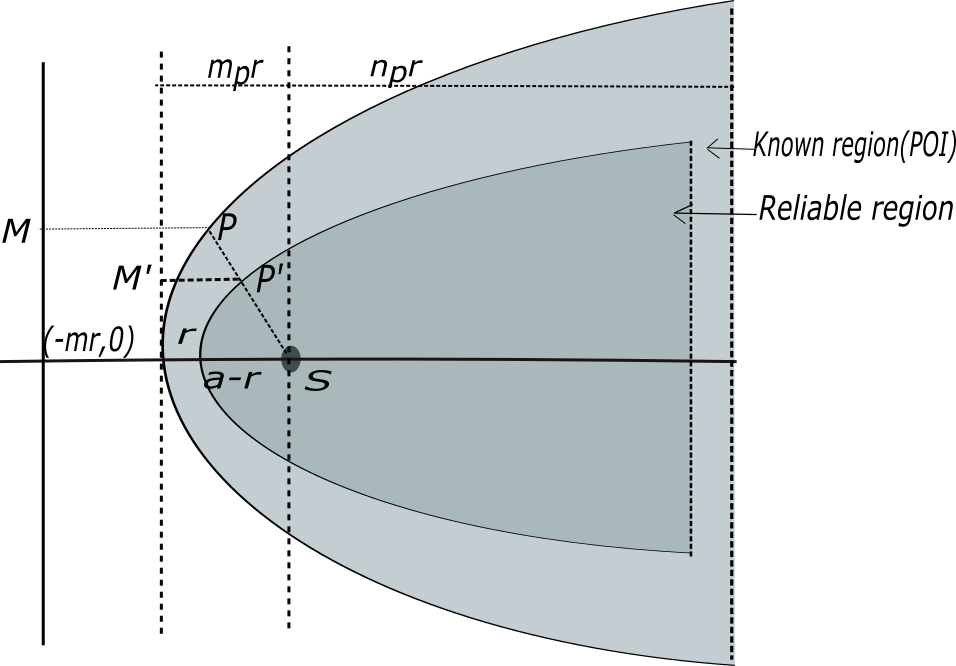
\includegraphics[width=\linewidth]{proof1.png}
  \caption{Proof for Theorem \ref{proofrel} }
  \label{fig:proof}
\end{figure}


\begin{theorem}
No computation is needed other than location calculation inside the safe region.
\end{theorem}

\begin{proof}
Since the safe region is a sub-set of the reliable region, so by the proof-1, no server query is needed to compute the answer set while the client is inside the safe region.

Now, by the construction of the safe region, the maximum Euclidean range of the safe region is, $r_{safe} = min_{\forall p \in P} dist_E(p, q) - r$. Therefore, even the next closest to be alarmed POI will not be missed even if no calculation is done while the cleint is inside the safe region.\\
However, the client's location $q$ must be regularly computed to check whether the safe region is crossed or not. Therefore, it is proved that no computation is needed other than location calculation inside the safe region.
\end{proof} 